
\Section{Schemes}
後できちんとした定義を述べるが,スキーム(scheme)とは局所環付き空間で局所的にはアフィンスキーム(affine scheme)とみれる
空間のことである.すなわち,先にアフィンスキームを定義せねばなるまい.\\
まず,$A$を環とし$X=\spec{A}$とし,Zariski位相が与えられてるとする.
このとき,$X$上の層$\mathcal{O}_{X}$を構成しよう.\\
まず,$D(f)\subset X$に対して$\mathcal{O}_{X}(D(f)) = A_{f}(=A[1/f])$とする.
次に射$\rho_{D(f),D(g)}:\mathcal{O}_{X}(D(f)) \to \mathcal{O}_{X}(D(g))$を定義しよう.\\
まず,$D(g) \subset D(f)$とする.つまり
\begin{equation*}
  g\in \sqrt{fA}
\end{equation*}
である.これは
\begin{equation}
  \exists m \in \mathbf{N}-\{0\},\exists b\in A\text{ s.t. } g^{m} = fb
\end{equation}
を意味する.よって$f$は$A_{g}$で単元である.実際上の式に両辺$1/g^{m}$をかけることによって
\begin{equation*} 
  f^{-1} = b/g^{m}
\end{equation*}
を得る.これによって制限写像$A_{f} \to A_{g}$を
\begin{equation*}
  a/f^{n} \mapsto ab^{n}/g^{mn}
\end{equation*}
で定義できる.もし$D(f) = D(g)$なら$A_{f} \to A_{g}$は同型射になる.(計算すれば容易にわかる.)
従って,$\mathcal{O}_{X}(D(f))$は$f$の選び方に依らない.$\{D(f)\}_{f}$は有限交叉で閉じた開基で
あったから,これは$\mathfrak{B}\text{-presheaf}$である.
\Proposition{
  $A$を環、$X=\text{Spec}\, A$とする。このとき以下が成り立つ。
  \begin{itemize}
    \item[(1)] $\mathcal{O}_{X}'$を環の$\mathfrak{B}$-層とする。$\mathcal{O}_{X}'$が誘導する$X$上の層$\mathcal{O}_{X}$は$\mathcal{O}_{X}(X)=A$となる。
    \item[(2)] 任意の$\mathfrak{p}\in X$に対して、茎$\mathcal{O}_{X,\mathfrak{p}}$は$A_{\mathfrak{p}}$への標準的な同型がある。特に、$(X,\mathcal{O}_{X})$は局所環付き空間になる。
  \end{itemize}
}{
  まず,開集合$U=X$についてUniquness条件を確認する.ほかの基本開集合も同様に示される.
  $U_{i} = $
}

\Definition{
上で定義した局所環付き空間$(\text{Spec}\, A,\mathcal{O}_{\text{Spec}\, A})$を
\index{あふぃんすきーむ@アフィンスキーム}\index{affine scheme}
\textbf{アフィンスキーム(affine scheme)}という.
}

\Example{
  環$R$に対して$\mathbf{A}_{R}^{n}:=\spec{R[X_{1},\cdots,X_{n}]}$とおく.
  これを\textbf{$R$上の相対次元$n$のアフィン空間(affine space of relative dimension $n$ over $R$)}という.
  もちろん$(\mathbf{A}_{R}^{n},\mathcal{O}_{\mathbf{A}_{R}^{n}})$はアフィンスキーム
}{}

\Lemma{
  $A$を整域とし$K$をその商体とする.素イデアル$0$に対応する$X = \text{Spec}\, A$の点を$\xi$とする.このとき
  \begin{equation*}
    \mathcal{O}_{X,\xi} = K
  \end{equation*}
  が成り立つ.さらに,任意の空でない開集合$U \subset X$と$\xi \in U$に対して標準的な準同型
  \begin{equation*}
    \mathcal{O}_{X}(U) \to \mathcal{O}_{X,\xi}
  \end{equation*}
  は単射となる.開集合の組$V \subset U$に対して制限
  \begin{equation*}
    \mathcal{O}_{X}(U) \to \mathcal{O}_{X}(V)
  \end{equation*}
  は単射となる.
}{
  Prop:\ref{Prop:1.5.1}(2)より
  \begin{equation*}
    \mathcal{O}_{X,\xi} = A_{\xi} = K
  \end{equation*}
  を得る.\\
  $U=D(f)$とすると,$\mathcal{O}_{X}(U) = A_{f}\subset K$.一般に
  \begin{equation*}
    U = \bigcup_{i}D(f_{i})
  \end{equation*}
  と置く.$s\in \mathcal{O}_{X}(U)$を飛ばすと$0 \in K$になるとする.各開被覆$D(f_{i}) \subset U$への
  制限を考えると
  \begin{equation*}
    s|_{D(f_{i})} = 0
  \end{equation*}
  が任意の$i$で成り立つので,$s=0$である.よって$\mathcal{O}_{X}(U) \to \mathcal{O}_{X,\xi} \subset K$は単射.\\
  開集合の組$\xi \in V\subset U$に対して制限$\mathcal{O}_{X}(U) \to \mathcal{O}_{X}(V)$に対して帰納極限の定義より図式
  \begin{center}
    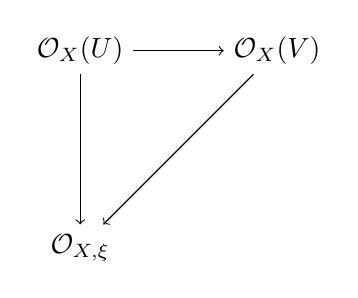
\begin{tikzpicture}[auto]
      \node (OU) at (0,0) {$\mathcal{O}_{X}(U)$};
      \node (Oxi) at (0,-2.5) {$\mathcal{O}_{X,\xi}$};
      \node (OV) at (2.5,0) {$\mathcal{O}_{X}(V)$};
      \node (ci) at (0.75,-0.75) {$\circlearrowleft$};

      \draw[->] (OU) to node () {} (OV);
      \draw[->] (OU) to node () {} (Oxi);
      \draw[->] (OV) to node () {} (Oxi);
    \end{tikzpicture}
  \end{center}
  が可換となるので,制限は単射である.
}

\Lemma{
$X = \text{Spec}\, A$をアフィンスキームとし,$g\in A$をとる.このとき開集合$D(g)$は
$X$から誘導される局所環付き空間で$\spec{A_{g}}$に同型なアフィンスキームになる.
}{
$Y = \spec{A_{g}}$と置く.局所化と素イデアルの対応より標準的な開はめ込み
\begin{equation*}
  i:Y \to X
\end{equation*}
がある($\im i = D(g)$)\\
$D(h)\subset D(g)$とする.$A\stackrel{\varphi}{\longrightarrow} A_{g}$とする.また$\varphi(h) = \bar{h}$と置く.このとき標準的な同型
\begin{equation*}
  \mathcal{O}_{X}(D(h)) = A_{h} \simeq (A_{g})_{\bar{h}} = \mathcal{O}_{Y}(D(\bar{h})) = i_{*}\mathcal{O}_{Y}(D(h))
\end{equation*}
今$A_{h}\simeq (A_{g})_{\bar{h}}$は感覚的には
\begin{equation*}
  (A_{g})_{\bar{h}} = (A[1/g])_{\bar{h}} = A[1/g,1/\bar{h}]
\end{equation*}
で,$D(h)\subset D(g)$より$h^{n} = gb$となる$n\in \mathbf{N}-\{0\}$と$b\in A$がある.よって
\begin{equation*}
  A[1/g,1/\bar{h}] = A[b/h^{n},1/\bar{h}] = A[1/h]=A_{h}
\end{equation*}
具体的にはまず,$\varphi$が単射ではないとき,
\begin{equation*}
  \ker{\varphi} \neq 0 \Leftrightarrow A_{g} = 0
\end{equation*}
に注意すると(よって$(A_{g})_{\bar{h}} = 0$),定義から$\ker{\varphi} \ni a \neq 0$とすると
\begin{equation*}
  \exists m\in \mathbf{N}\text{ s.t. } g^{m}a = 0
\end{equation*}
を満たす.また$h^n = gb$より$h^{nm}a = g^{m}ab^{m} = 0$より$\ker{(A\to A_{h})}$は$0$でない.
従って,$A_{h}=0$だから自明に同型である.よって$\varphi$を単射とする.\\
\begin{equation*}
  (A_{g})_{\bar{h}} \to A_{h}
\end{equation*}
を,
\begin{equation*}
  \frac{a}{g^{m}}\frac{1}{\bar{h}^{k}} \mapsto \frac{ab^{m}}{h^{mn}}\frac{1}{h^{k}} = \frac{ab^{m}}{h^{mn + k}}
\end{equation*}
で定義する.これは簡単に準同型で$0\leq k<n$としてよい.次に
\begin{equation*}
  A_{h} \to (A_{g})_{\bar{h}}
\end{equation*}
を,
\begin{equation*}
  \frac{a}{h^{n}} \mapsto \frac{\bar{a}}{\bar{h}^{n}}
\end{equation*}
ただし,$0\leq k<n$とする.これらは互いに逆射を与えるので,
$\{D(h)\}_{h}$は$D(g)$の開基となるので,$i$は$(Y,\mathcal{O}_{Y})$から$(D(g),\mathcal{O}_{X}|_{D(g)})\subset (X,\mathcal{O}_{X})$
への同型を誘導する.(Refer to Exercises 2.7)
}

\Definition{
\index{すきーむ@スキーム}\index{scheme}
\textbf{スキーム(scheme)}とは局所環付き空間$(X,\mathcal{O}_{X})$で開被覆$\{U_{i}\}_{i}$に対して$(U_{i},\mathcal{O}_{X}|_{U_{i}})$
がアフィンスキームになるものが存在するときをいう.また$\mathcal{O}_{X}(U)$の元は(やや不適切であるが)
\index{せいそくかんすう@正則関数}\index{regular function}
\textbf{$U$上の正則関数(regular functions on $U$)}という.しかし,層の関数としての側面をよく表している.(Refer to Exercises 3.4 and Proposition 4.4)
}

明らかにアフィンスキームはスキームである.また,局所環付き空間$X$が開被覆$\{U_{i}\}_{i}$に対して
$(U_{i},\mathcal{O}_{X}|_{U_{i}})$がスキームだったら$X$はスキームである.逆に次の命題が従う.

\Proposition{
$X$をスキームとする.このとき任意の開集合$U\subset X$に対して局所環付き空間$(U,\mathcal{O}_{X}|_{U})$はまたスキームになる.
}{
定義より$X = \bigcup_{i}U_{i}$で$U_{i}$は開集合で,アフィンスキームになるものがある.
$U\cap U_{i}$がスキームとなることを示せば十分である.
}

\Definition{
$X$をスキームとする.$U$を$X$の開集合とする.スキーム$(U,\mathcal{O}_{X}|_{U})$を$X$の
\index{かいぶぶんすきーむ@開部分スキーム}\index{open subscheme}
\textbf{開部分スキーム(open subscheme)}
更に$(U,\mathcal{O}_{X}|_{U})$がアフィンスキームになるとき$U$を
\index{あふぃんかいしゅうごう@アフィン開集合}\index{affine open subset}
\textbf{アフィン開集合(affine open subset)}という.
}

以下,$X$の開集合$U$はスキームの構造が与えられているとする.

\Definition{
  $X$をスキーム,$f\in \mathcal{O}_{X}(X)$とする.
  \begin{equation*}
    X_{f}:= \{x\in X\ |\ f_{x} \in \mathcal{O}^{\times}_{X,x}\}
  \end{equation*}
  ただし,$A^{\times}$は$A$の単元群である.(LiuのDefinition 3.11.では*の記号を用いている.)
}

次の条件を考えよう.

\begin{conditionbox}
  $X$は有限アフィン開被覆$\{U_{i}\}_{i}$があって$U_{i}\cap U_{j}$はまた有限アフィン開被覆を持つ.
\end{conditionbox}
便宜上この条件を条件Aと呼称する.



\Proposition{
$X$をスキームとし$f\in \mathcal{O}_{X}(X)$とする.このとき$X_{f}$は$X$の開集合で,
更に,$X$が条件Aを満たすなら,制限$\mathcal{O}_{X}(X)\to \mathcal{O}_{X}(X_{f})$は同型
\begin{equation*}
  \mathcal{O}_{X}(X)_{f} \simeq \mathcal{O}_{X}(X_{f})
\end{equation*}
を誘導する.
}{
$x\in X_{f}$とする.$x$の開近傍$U$と$g\in \mathcal{O}_{X}(U)$があって,$f_{x}g_{x} = 1$を満たすものがある.
$f_{x}g_{x} = (fg)_{x}$よりある$x$の開近傍$V\subset U$があって$fg|_{V}=1$を満たす.
したがって,$V\subset X_{f}$となる.よって$X_{f}$は開集合である.\\
更に,$V$が動くにつれて$f$の逆元$g\in \mathcal{O}_{X}(V)$を張り合わせると
$f|_{X_{f}}$の$\mathcal{O}_{X}(X_{f})$での逆元を得る.\\
詳しく言えば,$X_{f}$の上の$V$を集めた開被覆$\{V_{i}\}_{i}$を取り,$fg_{i}|_{V_{i}} = 1$なる$g_{i} \in \mathcal{O}_{X}(V_{i})$を考えれば
任意の$i,j$に対して
\begin{equation*}
fg_{i}|_{V_{i} \cap V_{j}} = 1 = fg_{j}|_{V_{i} \cap V_{j}}
\end{equation*}
より
\begin{align*}
(左辺) - (右辺) 
&= fg_{i}|_{V_{i} \cap V_{j}} - fg_{j}|_{V_{i} \cap V_{j}}\\
&= f|_{V_{i} \cap V_{j}}(g_{i}|_{V_{i} \cap V_{j}} - g_{j}|_{V_{i} \cap V_{j}})\\
&= 0
\end{align*}
また,$f|_{V_{i}}$は単元なので逆元$(f|_{V_{i}})^{-1}$がある.また,
\begin{equation*}
f|_{V_{i} \cap V_{j}} = (f|_{V_{i}})|_{V_{i} \cap V_{j}}
\end{equation*}
なので,
\begin{align*}
f|_{V_{i} \cap V_{j}} ((f|_{V_{i}})^{-1}|_{V_{i} \cap V_{j}}) 
&= (f|_{V_{i}})|_{V_{i} \cap V_{j}} ((f|_{V_{i}})^{-1}|_{V_{i} \cap V_{j}}) \\
&= ((f|_{V_{i}})(f|_{V_{i}})^{-1})|_{V_{i} \cap V_{j}} \\
&= 1
\end{align*}
よって$f|_{V_{i} \cap V_{j}}$はまた単元で$g_{i}|_{V_{i} \cap V_{j}} = g_{j}|_{V_{i} \cap V_{j}}$を得る.

$\mathcal{O}_{X}$は層なので,貼り合わせ条件より$g|_{V_{i}} = g_{i}$なる$g\in \mathcal{O}_{X}(X_{f})$がある.
この$g$が$f|_{X_{f}}$の逆元になっている.\\
よって制限$\mathcal{O}_{X}(X)\to \mathcal{O}_{X}(X_{f})$
から準同型
\begin{equation*}
\alpha : \mathcal{O}_{X}(X)_{f}\to \mathcal{O}_{X}(X_{f});\frac{x}{f^n} \mapsto \rho_{X,X_f}(x)f^{-n} = \rho_{X,X_f}(x)g^n
\end{equation*}
を誘導する.($\mathcal{O}_{X}(X)$は環なので$\mathcal{O}_{X}(X)_{f}$は$\{f^{n}\}_{n\in \mathbf{N}}$での局所化であることに注意しよう.)
ここで条件Aを仮定すれば,$X$は有限アフィン開被覆$\mathcal{U} = \{U_{i}\}_{i}$を持つ.
よって,
\begin{equation*}
X_{f} = \bigcup_{i}U_{i}\cap X_{f} = \bigcup_{i}V_{i} = \bigcup_{i}D(f|_{U_{i}})
\end{equation*}
ここで,$U_{i} = \spec{A_{i}}$とすると
\begin{align*}
  U_{i} \cap X_{f} 
  &= \{x\in X\cap \spec{A_{i}}\mid f_{x} \in \mathcal{O}_{X,x}^{\times}\}\\
  &= \{x\in \spec{A_{i}}\mid f_{x} \in \mathcal{O}_{X,x}^{\times}\}\\
  &= \{x\in \spec{A_{i}}\mid f_{x} \in (\mathcal{O}_{X}|_{\spec{A_{i}},x})^{\times}\}\\
  &= \{\mathfrak{p}\in \spec{A_{i}}\mid f_{\mathfrak{p}} \in A_{i,\mathfrak{p}}^{\times}\}
\end{align*}
ここで,素イデアルの局所化$A_{\mathfrak{p}}$が局所環でその極大イデアルが
$A_{\mathfrak{p}}\mysetminus A_{\mathfrak{p}}^{\times} = \mathfrak{p}A_{\mathfrak{p}}$となることに注意すると
\begin{align*}
  \{\mathfrak{p} \in \spec{A_{i}}\mid f_{\mathfrak{p}}\in A_{i,\mathfrak{p}}^{\times}\}
  &= \{\mathfrak{p} \in \spec{A_{i}} \mid f_{\mathfrak{p}} \notin \mathfrak{p}A_{i,\mathfrak{p}}\}\\
  &= \{\}
\end{align*}
%D(f|_{U_{i}})がなぞ
Lem:\ref{Lem:1.5.3}より$\mathcal{O}_{X}(U_{i})_{f} = \mathcal{O}_{X}(V_{i})$\\
今以下の完全系列を得る.
\begin{equation*}
C^{\bullet}(\mathcal{U},\mathcal{O}_{X}):0 \longrightarrow \mathcal{O}_{X}(X) \stackrel{d_{0}}{\longrightarrow} \bigoplus_{i}\mathcal{O}_{X}(U_{i}) \stackrel{d_{1}}{\longrightarrow} \bigoplus_{i,j}\mathcal{O}_{X}(U_{i} \cap U_{j})
\end{equation*}
ただし$d_{0}:s\mapsto (s|_{U_{i}})_{i},d_{1}:(s_{i})_{i}\mapsto (s_{i}|_{U_{i}\cap U_{j}} - s_{j}|_{U_{i} \cap U_{j}})_{i,j}$
とする.(有限個なら直積$\prod$と直和$\bigoplus$は同じ)\\
次にテンソルをとることは左完全関手なので$C^{\bullet}(\mathcal{U},\mathcal{O}_{X})\otimes_{\mathcal{O}_{X}(X)}\mathcal{O}_{X}(X)_{f}$
はまた,完全列である.よってこれは次の可換図式を与える.

\begin{center}
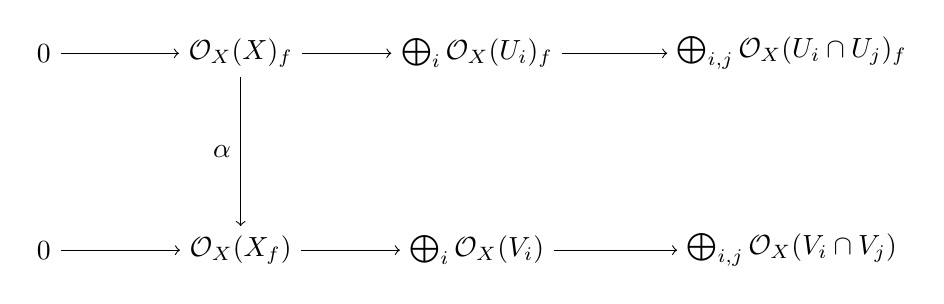
\begin{tikzpicture}[auto]
  \node (00) at (0,0) {$0$};
  \node (01) at (0,-2.5) {$0$};
  \node (OX_f) at (2.5,0) {$\mathcal{O}_{X}(X)_{f}$};
  \node (OXf_) at (2.5,-2.5) {$\mathcal{O}_{X}(X_{f})$};
  \node (oOU_f) at (5.5,0) {$\bigoplus_{i}\mathcal{O}_{X}(U_{i})_{f}$};
  \node (oOV) at (5.5,-2.5) {$\bigoplus_{i}\mathcal{O}_{X}(V_{i})$};
  \node (oOUU_f) at (9.5,0) {$\bigoplus_{i,j}\mathcal{O}_{X}(U_{i}\cap U_{j})_{f}$};
  \node (oOVV) at (9.5,-2.5) {$\bigoplus_{i,j}\mathcal{O}_{X}(V_{i}\cap V_{j})$};
  \node (ci) at (1.25,-1.25) {$\circlearrowleft$};

  \draw[->] (00) to (OX_f);
  \draw[->] (01) to (OXf_);
  \draw[->] (OX_f) to (oOU_f);
  \draw[->] (OXf_) to (oOV);
  \draw[->] (oOU_f) to (oOUU_f);
  \draw[->] (oOV) to (oOVV);
  \draw[->] (OX_f) to node[label=left:$\alpha$] () {} (OXf_);
  % \draw[->] (X2) to node[yshift = -2pt,label=below:$f_{\lambda}$] () {} (Y2);
  % \draw[->] (Y1) to node[xshift = -6pt,label=right:$\psi_{\lambda,\mu}$] () {} (Y2);
\end{tikzpicture}
\end{center}
}